\section{Concepts}\label{section:prototype}
In this section concepts will be illustrated. 
The concepts will be used as a draft before implementing the final application, where the state diagram \figref{figure:state-diagram} is used to derive the layout.

The user is first presented with the \textit{Main Menu}, which can be seen in \figref{figure:main-menu}.
The Main Menu will enable the user to start the game and view the \textit{High score}.
In the High score, \figref{figure:highscore}, the user can see a list of scores achieved on the phone.

\begin{figure}[H]
	\centering
	\begin{subfigure}[b]{0.3\textwidth}
	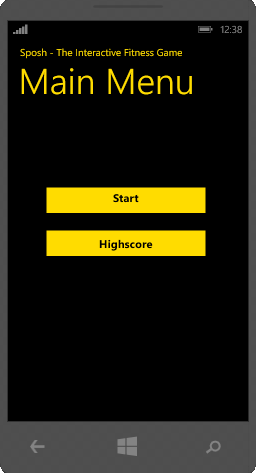
\includegraphics[scale = 0.55]{media/prototype/main-menu.png}
	\caption{Main Menu}
	\label{figure:main-menu}
	\end{subfigure}
	\qquad
	\begin{subfigure}[b]{0.3\textwidth}
	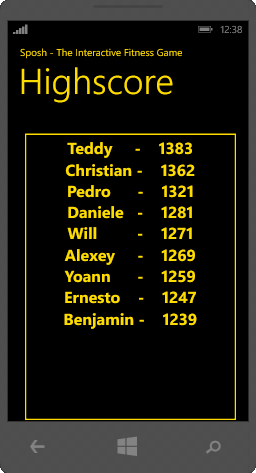
\includegraphics[scale = 0.55]{media/prototype/highscore.png}
	\caption{High score}
	\label{figure:highscore}
	\end{subfigure}
	\caption{The prototype of the Main Menu(\textit{a}) and the High score (\textit{b})}
\end{figure}
In \figref{figure:thegame}, the user plays the game. 
In this screen the borders of the game, the ball, and the paddle can be seen.
When the ball has passed the paddle, the user loses the game and is taken to the score screen, where the user can save his score, replay the game, or return to the main menu, as can be seen in \figref{figure:score-screen}.

\begin{figure}[H]
	\centering
	\begin{subfigure}[b]{0.4\textwidth}
	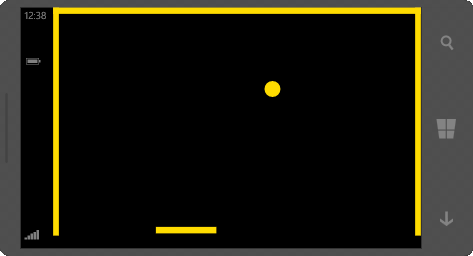
\includegraphics[scale = 0.5]{media/prototype/game.png}
	\caption{The Game.}
	\label{figure:thegame}
	\end{subfigure}
	\qquad
	\begin{subfigure}[b]{0.4\textwidth}
	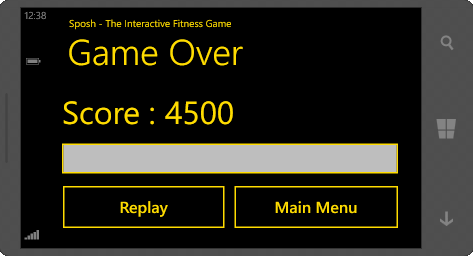
\includegraphics[scale = 0.5]{media/prototype/score-screen.png}
	\caption{The Score Screen.}
	\label{figure:score-screen}
	\end{subfigure}
	\caption{The game (\textit{a}) and the score screen (\textit{b})}
\end{figure}
